% Rapport sur l'environnement de développement avec Vagrant
\documentclass[12pt,a4paper]{article}

\usepackage[francais]{babel}
\usepackage[utf8]{inputenc}
\usepackage[T1]{fontenc}
\usepackage{graphicx} % Pour intégrer des images
\usepackage{hyperref} % Liens externes
\usepackage{listings} % Code source
\usepackage{hyperref} % Lien hypertexte

\usepackage{vmargin} % Pour formater la taille des marges du doc
\setpapersize{A4}
\setmargins{20mm}{15mm}{170mm}{250mm}{10mm}{0mm}{0pt}{1.2cm}

\title{Les environnements de développement avec Vagrant et Docker}
\author{Maxence Bothorel, Thibaut Crouvezier}
\date{22/01/2015}

\lstset{literate=
	{á}{{\'a}}1 {é}{{\'e}}1 {í}{{\'i}}1 {ó}{{\'o}}1 {ú}{{\'u}}1
	{Á}{{\'A}}1 {É}{{\'E}}1 {Í}{{\'I}}1 {Ó}{{\'O}}1 {Ú}{{\'U}}1
	{à}{{\`a}}1 {è}{{\`e}}1 {ì}{{\`i}}1 {ò}{{\`o}}1 {ù}{{\`u}}1
	{À}{{\`A}}1 {È}{{\'E}}1 {Ì}{{\`I}}1 {Ò}{{\`O}}1 {Ù}{{\`U}}1
	{ä}{{\"a}}1 {ë}{{\"e}}1 {ï}{{\"i}}1 {ö}{{\"o}}1 {ü}{{\"u}}1
	{Ä}{{\"A}}1 {Ë}{{\"E}}1 {Ï}{{\"I}}1 {Ö}{{\"O}}1 {Ü}{{\"U}}1
	{â}{{\^a}}1 {ê}{{\^e}}1 {î}{{\^i}}1 {ô}{{\^o}}1 {û}{{\^u}}1
	{Â}{{\^A}}1 {Ê}{{\^E}}1 {Î}{{\^I}}1 {Ô}{{\^O}}1 {Û}{{\^U}}1
	{œ}{{\oe}}1 {Œ}{{\OE}}1 {æ}{{\ae}}1 {Æ}{{\AE}}1 {ß}{{\ss}}1
	{ç}{{\c c}}1 {Ç}{{\c C}}1 {ø}{{\o}}1 {å}{{\r a}}1 {Å}{{\r A}}1
	{€}{{\EUR}}1 {£}{{\pounds}}1
}

\begin{document}

\maketitle{}

\begin{center}
  
\includegraphics[width=10cm]{images_rapport/univ_logo.jpg}
\end{center}

\newpage{}

\tableofcontents{}

\newpage{}

\section{Introduction}
Un environnement de développement est un ensemble d'outils et de logiciels afin d'augmenter la productivité d'un développeur. Cela peut être un éditeur de texte, avec un débogeur et un compilateur. Dans notre cas, l'environnement de développement est une plateforme qui sert au développeur à essayer ses logiciels, dans un environnement cloturé afin de ne pas porter atteinte à son système en cas d'erreurs. L'environnement est de préférence portable, afin que plusieurs développeurs puissent travailler avec la même base. Nous verrons deux pionniers dans le domaine : Vagrant et Docker. Nous étudierons leurs utilisations et leurs configurations après avoir rappelé leurs concepts, la virtualisation et les conteneurs. 

\section{Rappels}

\subsection{Qu'est-ce que la virtualisation ?}

La virtualisation est le fait de créer une "machine virtuelle", un nouveau système d'exploitation qui s'exécutera au dessus du système principal. On dit que la machine hôte est celle où la machine invitée est virtualisée. Cette machine virtuelle est indépendante du matériel.

Le système invité est entièrement indépendant de l'hôte, ce qui permet de virtualiser un Microsoft Windows 7 sur Debian 8, ou l'inverse. Ce système a ses limites. En effet, il est gourmand en ressources (processeur, RAM) puisqu'il faut disposer d'assez de puissance pour faire fonctionner plusieurs systèmes d'exploitations.

\begin{center}
  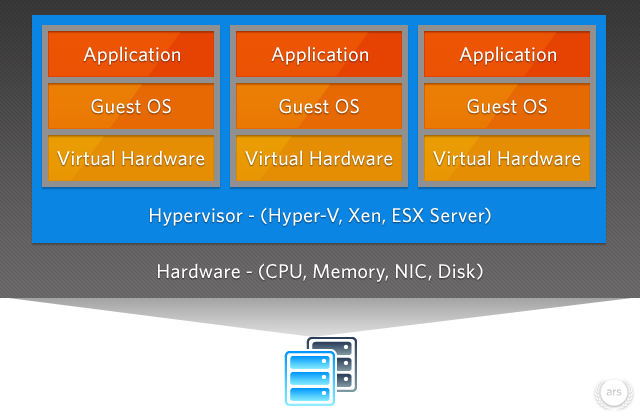
\includegraphics[width=15cm]{images_rapport/virtualisation.jpg}
\end{center}

Sur l'image ci-dessus, on peut voir le matériel en gris, puis l'hyperviseur en bleu, c'est à dire le système hôte. On voit également qu'il y a trois systèmes invités, avec leurs applications. On voit clairement que les systèmes invités sont indépendants du matériel de la machine, puisqu'il est également virtualisé. On peut décider de créer un ensemble de matériels virtuels, comprenant un disque dur virtuel de 20Go, un processeur avec 2 coeurs et 4Go de RAM afin qu'une machine puisse fonctionner.

\subsection{Qu'est-ce que la virtualisation par conteneurs ?}

La virtualisation par conteneurs ne nécessite pas de virtualiser un système d'exploitation complet, il se charge juste d'empaqueter un environnement de développement léger pour le déploiement d'applications. Ce système de virtualisation est dépendant du système hôte et des conteneurs entre eux. 

\begin{center}
  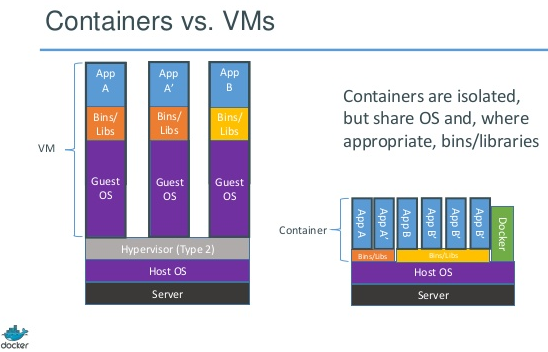
\includegraphics[width=15cm]{images_rapport/vm_container.jpg}
\end{center}

Le désavantage de cette virtualisation est qu'elle se base sur le noyau du système hôte, ce qui restreint son déploiement. Il faut donc un conteneur Linux pour un noyau Linux. 

De l'autre coté, cette dépendance au noyau, permet une meilleure gestion des ressources. En effet, la virtualisation par conteneurs permet de pouvoir exploiter toute la quantité de RAM de l'hôte, ainsi que tous les coeurs de son processeur.

\section{Vagrant}

\subsection{Introduction}
\begin{center}
  
\includegraphics[width=12cm]{images_rapport/vagrant_logo.jpg}
\end{center}

\textbf{Vagrant} est un outil développé en Ruby, sous licence MIT pour créer des environnements de développements. Il se veut simple d'utilisation afin d'augmenter la productivité de l'utilisateur. Le développement de Vagrant à commencé en Janvier 2010 par Mitchell Hashimoto. Celui ci a travaillé sur Vagrant pendant 3 ans sur son temps libre, avant de créer l'entreprise \textbf{Hashicorp}, afin de continuer le projet à plein temps.

Vagrant créé et gère des machines virtuelles à destinations des développeurs. Ces machines permettent à l'utilisateur d'effectuer des tests dans un environnement fermé, afin de ne pas affecter son système d'exploitation principal. 

Vagrant met en place des machines virtuelles sur VirtualBox, VMWare (Fusion et Workstation), dans le cloud grâce à AWS d'Amazon et Openstack, et également dans des conteneurs Docker et LXC. Il est disponible sur Windows, OS X et Linux. De plus, Red Hat a créé un plugin permettant à Vagrant de fonctionner avec KVM.

Vagrant permet donc de travailler de façon sécurisée, à seul ou à plusieurs afin d'essayer des logiciels, des scripts ou autre...

\subsection{Installation}
Vagrant est dans les dépôts de Debian unstable en version 1.6.5 et est disponible en version 1.7.2 sur le site officiel. Le projet Fedora ne supporte pas encore Vagrant. Malgré cela, les développeurs de Fedora souhaitent le proposer pour la version 22 avec le logiciel libvirt comme hyperviseur par défaut, au lieu de VirtualBox.

On peut donc télécharger le tarball sur GitHub, le récupérer grâce aux dépôts sur Debian et ses dérivés. On peut également télécharger les paquêts Deb, RPM, les éxecutables .msi et .dmg pour Windows et OS X sur le site officiel du projet.

Nous avons utilisé les versions disponible sur Debian unstable et la dernière, disponible sur le site officiel.

\subsection{Utilisation basique}

Pour créer une nouvelle machine virtuelle, il suffit d'utiliser les commandes :
\begin{lstlisting}
vagrant init ubuntu/trusty64
vagrant up
vagrant ssh
\end{lstlisting}

La première commande sert à créer un Vangrantfile, un fichier de configuration de la machine. La deuxième commande télécharge le disque virtuel hébergé par l'Atlas d'Hashicorp\footnote{Hashicorp a créé un \href{https://atlas.hashicorp.com/boxes/search}{annuaire de machines}, l'Atlas, afin de faciliter les téléchargements}, la société derrière Vagrant.
Au bout de quelques minutes, la machine est téléchargée et prête à être utilisée. Un shell est lancé grâce à la dernière commande. 

Lorsqu'une commande de Vagrant est utilisée, celui-ci remonte l'arborescence afin de trouver le Vagrantfile. On peut changer le répertoire à partir duquel Vagrant lance la recherche grâce à la variable d'environnement VAGRANT\_CWD. 

\subsection{Fichiers de configuration}
Les fichiers de configuration de Vagrant sont des Vagrantfiles. Il en existe plusieurs, et sont tous lus dans un certain ordre lors du démarrage d'une machine :
\begin{enumerate}
	\item{Le Vagrantfile téléchargé avec la machine.}
	\item{Un Vagrantfile dans le dossier /home/user/.vagrant.d, qui est appliqué sur toutes les machines.}
	\item{Le Vagrantfile créé lors de la commande d'initialisation de la machine.}
	\item{Si le dernier n'existe pas, un Vagrantfile concernant plusieurs machines.}
	\item{Si le dernier n'existe pas non plus, un Vagrantfile qui concerne l'hyperviseur.}
\end{enumerate}

Les fichiers sont donc lus un par un et les configurations fusionnées ou remplacées. C'est du Ruby (ce qui permet d'en faire des scripts aisément) :
\begin{lstlisting}
Vagrant.configure(2) do |config|
  ...
end
\end{lstlisting}
Toutes les configurations se retrouvent entre ces deux lignes. Le chiffre 2 signifie que la version de configuration est pour Vagrant version 1.1 ou plus, alors que les configurations pour les versions 1.0.x sont mentionnées par un 1.

On peut également obliger l'utilisateur à avoir une certaine version de Vagrant (dans ce cas, une version entre la 1.3.5 et la 1.4.0) :
\begin{lstlisting}
Vagrant.require_version ">= 1.3.5", "< 1.4.0"
\end{lstlisting}

Il existe beaucoup de paramètres de configurations et sont classés comme ceci : 
\begin{itemize}
	\item{Les configurations comprenant config.vm, qui concernent la machine et son disque virtuel (mise à jour, checksum, réseau, hostname...).}
	\item{Les configurations comprenant config.ssh, qui permet à Vagrant de savoir comment utiliser SSH avec la machine (port, clé SSH, utilisation de X11...).} 
	\item{Les configurations comprenant config.winrm, qui permettent à Vagrant de savoir comment accéder à une machine Windows (nom d'utilisateur, mot de passe, port...).}
	\item{Les configurations comprenant config.vagrant, qui concernent le système hôte. Par défaut en détection automatique.}
\end{itemize}
En voici quelques exemples :
\begin{lstlisting}
config.vm.network "forwarded_port", guest: 80, host: 8080 
# Pour rediriger le port 8080 de l'hôte vers le port 80 de l'invité
config.vm.network "private_network", type: "dhcp" 
# Activer une nouvelle interface en mode DHCP
config.ssh.username
# Change le nom d'utilisateur lors de la commande vagrant ssh
config.ssh.private_key_path
# Change la clé privée qu'utilise SSH
config.winrm.host
# L'adresse IP à laquelle se connecter (pour Windows)
\end{lstlisting}

\subsection{Partages}

\subsubsection{Le partage de dossier}
Vagrant permet de partager des dossiers entre l'hôte et l'invité. De base, le dossier partagé est celui où est le Vagrantfile sur l'hôte, et /vagrant sur l'invité. Le type de partage par défaut est celui de VirtualBox si l'on utilise ce logiciel, mais d'autres existent.

La commande pour la synchronisation des dossiers dans le Vagrantfile est\footnote{Le paramètre a été mis sur deux lignes pour éviter qu'il déborde de la page} :
\begin{lstlisting}
 config.vm.synced_folder "src/", "/srv/website", 
   create: true, disabled: false, type: nfs
\end{lstlisting}
On peut voir ci-dessus que lors du prochain redémarrage de la machine :
\begin{itemize}
	\item{Le dossier src/ de l'hôte sera synchronisé avec le dossier /srv/website de l'invité.}
	\item{Le dossier de la machine hôte sera créé s'il n'existe pas.}
	\item{Le partage sera activé.}
	\item{Le type de partage sera NFS.}
\end{itemize}
Il existe également les paramètres pour définir le propriétaire du partage, le groupe du partage (tous deux SSH par défaut), et les options de montages.

De plus, d'autres paramètres existent pour le partage NFS : 
\begin{itemize}
	\item{nfs\_export (booléen) : S'il est a false, vagrant ne modifiera pas le fichier /etc/exports utilisé par NFS.}
	\item{nfs\_udp (booléen) : Ce paramètre sert à savoir quel protocole de transport utilisé.}
	\item{nfs\_version (nombre) : Ce paramètre sert à déterminer la version de NFS utilisé.}
\end{itemize}
Pour que Vagrant modifie le fichier /etc/exports utilisé par NFS, il lui faut des droits root. Il est donc possible de renseigner le mot de passe à chaque démarrage de machine, de mettre vagrant dans le groupe sudoers ou de modifier soi-même le fichier.

Il est également possible de partager les dossiers avec rsync. Dans ce cas, il sera nécessaire d'utiliser rsync-auto afin de synchroniser les dossiers à chaque changements. Le partage via SMB est quant à lui disponible que pour les hôtes Windows. 

Le partage via NFS est à privilégier car il est plus performant et a moins d'inconvéniants (un bug de VirtualBox peut entraîner des fichiers corrompus, la synchronisation automatique avec rsync est plus fastidieuse a mettre en place et SMB n'est disponible que pour les hôtes Windows).

\subsubsection{Le partage des machines}
Vagrant est un logiciel collaboratif : il est possible de faire profiter de ses machines avec n'importe qui. Pour ce faire, il faut créer un compte sur le site Atlas de Vagrant et de s'y connecter avec \textit{vagrant login}. Ensuite, il suffit de lancer ces commandes :
\begin{lstlisting}
vagrant share
\end{lstlisting}

Cette commande lance le partage. Sans options, tous les ports disponibles de la machine invitée sont partagés. Le résultat est une URL de la forme "http://nom.vagrantshare.com". Elle pointe vers Vagrant installé sur la machine hôte, qui a une redirection vers l'invité. Le HTTPS peut être activé grâce au paramètre --https.

On peut voir sur l'image suivante que le partage est lancé, et qu'un client est connecté grâce à l'URL fournie par Vagrant.

\begin{center}
	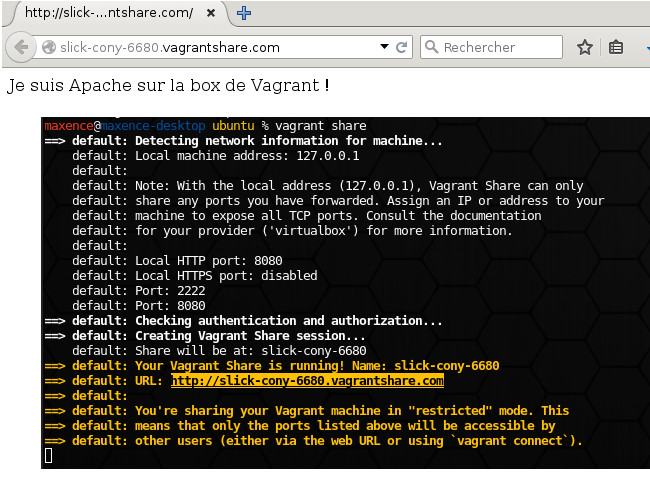
\includegraphics[width=13cm]{images_rapport/sharehttp.jpg}
\end{center}

Le partage via SSH fonctionne de la même manière, grâce à la commande :
\begin{lstlisting}
vagrant share --ssh
\end{lstlisting}
Cette fois-ci, seulement le nom du partage à fournir à un collègue est retourné :

\begin{center}
	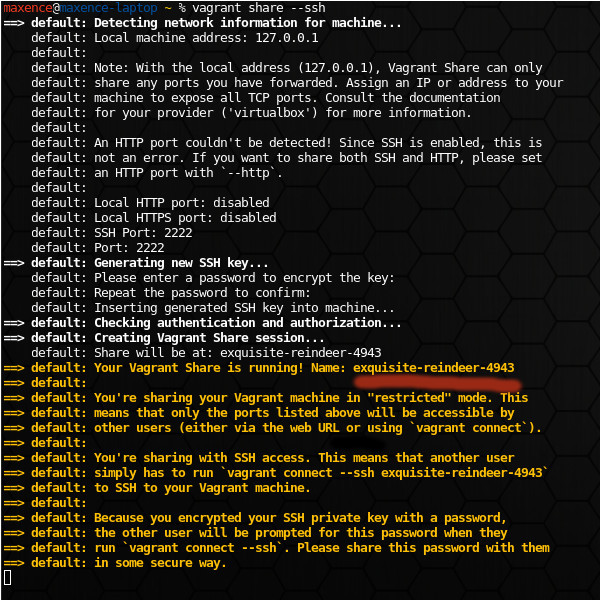
\includegraphics[width=12cm]{images_rapport/vagrantshare.jpg}
\end{center}

On peut voir sur cette image, que la machine virtuelle est bien partagée. Ainsi, il est possible pour quiconque connait le nom du partage, de s'y connecter : 

\begin{lstlisting}
vagrant connect --ssh exquisite-reindeer-4943
\end{lstlisting}

\begin{center}
	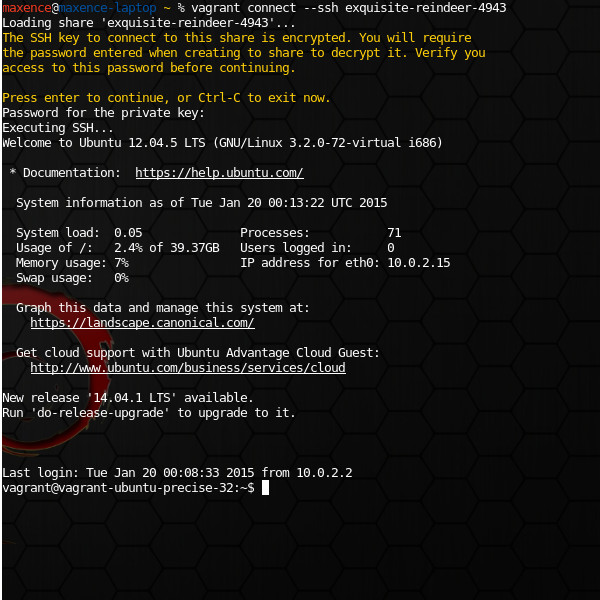
\includegraphics[width=12cm]{images_rapport/vagrantconnect.jpg}
\end{center}

La connexion s'effectue sans problèmes et le client est connecté en SSH sur la machine virtuelle. Ici, ce test a été effectué en local, mais il fonctionne également très bien à travers Internet.

Une autre possibilité est fort intéressante. Lorsque l'on partage une machine, un collaborateur peut effectuer la commande \textit{vagrant connect NAME} afin d'avoir une nouvelle adresse IP qui renvoie tous les flux TCP/IP vers la première machine virtuelle. Concrètement, la connection créé une machine virtuelle sur le poste du collaborateur, un proxy qui redirige toutes les connections vers la machine partagée. Cette nouvelle machine est très légère puisqu'elle consomme environ 20Mo de RAM sur VirtualBox ou VMWare. Par contre, il est vivement recommandé de changer les clés SSH qui sont avec le disque virtuel lors du téléchargement. En effet, quiconque connait le nom de la machine peut s'y connecter. 

Certains options permettent d'augmenter la sécurité de l'environnement de développement :
\begin{lstlisting}
--disable-http # Le partage HTTP n'est pas activé
--ssh-once     # Autorise qu'une seule connection SSH
\end{lstlisting}
La sécurité des VMs est également augmentée grâce à ces fonctionnalités :
\begin{itemize}
	\item{Le traffic est toujours chiffré à l'aide de TLS.}
	\item{Il existe quarante millions de noms différents pour le partage des machines.}
	\item{Lors d'un partage à travers SSH, la clé SSH est chiffée lors de la transmission.}
	\item{Les partages durent une heure, sauf si on la coupe manuellement avec ctrl-c.}
\end{itemize}

Hashicorp travaille actuellement sur l'ajout d'ACL et sur un moyen de changer les clés SSH automatiquement.	

\subsection{L'environnement "multi-machine"}
Le principe de l'environnement multi-machine est de configurer plusieurs systèmes avec un seul Vagrantfile, afin d'en faciliter la configuration. Dans le cas d'un projet comprenant plusieurs VMs, il peut être utile d'avoir toutes les configurations sous les yeux, en même temps.

\begin{lstlisting}
Vagrant.configure("2") do |config|
	config.vm.define "precise" do |precise|
		web.vm.box = "hashicorp/precise32"
		...
	end
	
	config.vm.define "trusty", autostart: false do |trusty|
		db.vm.box = "hashicorp/trusty64"
		...
	end
end
\end{lstlisting}
Réseau, partages, provisions... Les configurations des machines vont être dans "config.vm.define" au lieu d'être directement dans "Vagrant.configure". On peut ainsi mettre des configurations globales comme les provisions que nous verrons après. L'ordre de lecture des configurations est "Dehors, dedans". C'est à dire que Vagrant liste d'abord la configuration globale, puis celle de chaque machine.

	Le contrôle diffère un peu d'un projet ou une seule machine est utilisée. Bien que la commande \textit{vagrant up} démarrera toutes les machines, on peut définir le paramètre "autostart" qui empêchera le démarrage automatique. Dans ce cas, il faudra utiliser \textit{vagrant up nom\_machine} pour la démarrer. De même, il faudra utiliser \textit{vagrant ssh nom\_machine} afin de s'y connecter.

\subsection{Les provisions}

\subsubsection{Les provisions Shell}
La provision, avec Vagrant, permet d'installer automatiquement des logiciels ou de faire des configurations lors de la commande \textit{vagrant up}. 

Il faut indiquer les commandes à exécuter lors de la provision dans le Vagrantfile. Dans le cas de Linux, les scripts SHELL seront lancés à travers SSH, et grâce à WinRM et PowerShell dans le cas d'une machine Windows.
\begin{lstlisting}
config.vm.provision "apache", inline: <<-SHELL
	sudo apt-get update
	sudo apt-get install -y apache2
SHELL
\end{lstlisting}
Ainsi, toutes les commandes entre la première et dernière ligne seront éxecutées lors de l'appel de la provision. Ici, l'appel du nom "apache" lancera l'installation d'Apache2. En effet, on peut donner des noms différents aux provisions et les appeler individuellements :
\begin{lstlisting}
vagrant provision
vagrant provision provision-with apache sql  
vagrant up --no-provision
\end{lstlisting}
La première commande lancera toutes les provisions déclarées, la deuxième seulement les provisions apache et sql. Enfin, la dernière commande lance la machine sans exécuter de scripts.

Lorsque l'on utilise plusieurs machines, il peut être intéressant de regrouper les provisions de toutes celles-ci dans un même Vagrantfile. Pour les distinguer, on définie dans quelle machine on lance telle provision :
\begin{lstlisting}
config.vm.provision "mysql", type: "shell", 
	inline: "apt-get install mysql-server"

config.vm.define "web" do |web|
	web.vm.provision "php", 
		inline: "apt-get install php5"
	web.vm.provision "apache2", type: "shell", 
		inline: "apt-get install apache2"
end
\end{lstlisting}

Dans le cas ci-dessus, Apache2 et PHP5 seront installés seulement si la machine virtuelle s'appelle web. Sinon, mysql sera installé. Comme on l'a vu, on peut renseigner directement des commandes à exécuter, mais on peut également mettre un lien vers un script plus complexe. Dans ce cas, le paramètre "path" (qui prend comme valeur une chaîne de caractères) remplacera la paramètre "inline", vu plus haut. De plus, des arguments peuvent être précisés dans un tableau ou dans une chaîne de caractères.

\subsubsection{La provision File}
La provision appelée "file" permet d'envoyer un fichier vers le système invité. Cela fonctionne à travers SCP et cette provision prend en paramètre la source et la destination :
\begin{lstlisting}
config.vm.provision "file", source: "~/.zshrc", 
	destination: "~/.zshrc"
\end{lstlisting}

\subsubsection{Les provisions avec Docker}
Les provisions avec Docker peuvent installer automatiquement Docker, déployer, configurer et démarrer des conteneurs. Les provisions Docker peuvent être utilisées avec les autres sans problèmes. Il est par exemple possible d'installer des logiciels comme un SGBD, et de déployer avec Docker l'application qui utilisera cette base.

Il existe plusieurs options pour utiliser Docker dans Vagrant. Si aucune n'est renseignée, Vagrant installera juste Docker dans la machine virtuelle.

On peut d'abord créer un conteneur "monapplication" dans le répertoire "/mon/app" :
\begin{lstlisting}
config.vm.provision "docker" do |d|
    d.build_image "/mon/app",
		args: "-t 'monapplication'"
end
\end{lstlisting}

On peut aussi récupérer des images de Docker, disponible dans la catalogue de Docker, de façons différentes. La première télécharge une seule image donnée en paramètre :
\begin{lstlisting}
config.vm.provision "docker", images: ["nginx"]
\end{lstlisting}
La deuxième méthode, plus intéressante, utilise une fonction "pull\_images" qui télécharge les images données en paramètres à chaque fois qu'elle est appelée : 
\begin{lstlisting}
config.vm.provision "docker" do |d|
	d.pull_images "debian:jessie"
	d.pull_images "nginx"
end
\end{lstlisting}

Pour démarrer une image Docker, il faut utiliser "run" qui peut prendre des paramètres :
\begin{lstlisting}
config.vm.provision "docker" do |d|
	d.run "ubuntu",
		cmd: "bash -l",
	d.run "db-1", image: "mysql"
	d.run "db-2", image: "mysql"
end
\end{lstlisting}
Dans cet exemple, Docker démarrera le conteneur "ubuntu", en exécutant bash au démarrage. Les deux conteneurs db-1 et db-2 avec la même image "mysql".

\subsubsection{Autres}

D'autres types de provisions existent, comme Chef, Puppet, Salt, Ansible et CFEngine. Nous ne les détaillerons pas ici puisqu'il s'agit de logiciels complexes qui nécessitent de bien les connaître. Chaque logiciel est bien intégré à Vagrant puisqu'ils disposent de beaucoup d'options concernant les provisions.

\subsection{Créer ses propres machines}
Il peut être utile de créer ses propres boxes, afin de déployer ou partager ses machines. La commande diffère d'un hyperviseur à l'autre, 

Pour faire une machine de base à déployer sur l'Atlas, il est demandé :
\begin{itemize}
	\item{La première interface doit être "adapter1" et être en NAT}
	\item{De créer un utilisateur "vagrant" avec le mot de passe "vagrant".}
	\item{Que le mot de passe root soit "vagrant".}
	\item{Que sudo ne demande pas de mot de passe (pour que Vagrant puisse configurer le réseau et monter les dossiers partagés).}
	\item{De mettre l'option "UseDNS" à "no" dans le serveur SSH, afin d'augmenter la vitesse lorsque la machine n'est pas connectée à Internet}
	\item{D'installer les logiciels additionnels des hyperviseurs}
\end{itemize}

Afin d'empaqueter la machine, il faut utiliser la commande \textit{vagrant package --base nom\_machine} pour VirtualBox (ou le nom de la machine est celui utilisé par VirtualBox). Le contenu du .box créé doit être :
\begin{lstlisting}
Vagrantfile
box-disk1.vmdk
box.ovf
metadata.json
\end{lstlisting}

Dans le cas de VMWare, le disque virtuel doit être défragmenté avec \textit{vmware-vdiskmanager}, empaqueter à la main avec \textit{tar cvzf custom.box ./*} donc le contenu doit être :
\begin{lstlisting}
disk-s001.vmdk
disk-s002.vmdk
disk.vmdkmetadata.json
precise64.nvram
precise64.vmsd
precise64.vmx
precise64.vmxf
\end{lstlisting}

\subsection{Partager ses machines virtuelles}
Depuis la version 1.7, Vagrant permet de partager sa machine virtuelle à travers le réseau. On peut s'en servir pour la sauvegarder sur un serveur FTP, la donner à un collaborateur, et également la partager sur l'Atlas de Vagrant.

\subsubsection{Le partage FTP/SFTP}
Pour envoyer sa machine sur un serveur FTP ou SFTP, il faut rajouter une catégorie de configuration dans le Vagantfile :
\begin{lstlisting}
config.push.define "ftp" do |push|
	push.host = "ftp.mondomaine.com"
	push.username = "username"
	push.password = "password"
	push.secure = true
	push.destination = "/home/me"
	push.exclude = ".test"
end
\end{lstlisting}
Avec la configuration ci-dessus, on est capable d'envoyer sa machine virtuelle avec la commande \textit{vagrant push}. Dans ce cas, la machine sera envoyer en SFTP dans le dossier /home/me de la machine distante et le dossier ".test" ne sera pas envoyé.

\subsubsection{Le partage sur l'Atlas}
Pour l'envoyer sur l'annuaire des machines d'Hashicorp, le principe est le même :
\begin{lstlisting}
config.push.define "atlas" do |push|
  push.app = "mbothorel/debian8"
end
\end{lstlisting}
Il est également possible d'inclure ou d'exclure des dossiers à transférer, de modifier l'adresse de l'Atlas (par défaut l'Atlas public) ou encore d'utiliser un système de version de fichier pour déterminer les fichiers à envoyer.

\subsubsection{Stratégie locale}
De la même manière il est possible d'utiliser un script SHELL pour copier ou envoyer la machine.
\begin{lstlisting}
config.push.define "local-exec" do |push|
  push.inline = <<-SCRIPT
    scp . /var/www/website
	scp . user@host:~
  SCRIPT
end
\end{lstlisting}
On peut voir ci-dessus que les commandes entre les deux "SCRIPT" seront exécutées. C'est à dire la copie vers un répertoire local et la copie distante. Comme pour les provisions, la syntaxe accepte aussi le chemin vers un script :
\begin{lstlisting}
config.push.define "local-exec" do |push|
  push.script = "~/mon\_script.sh"
end
\end{lstlisting}

\section{Docker}

\subsection{Introduction}
\begin{center}
  
\includegraphics[width=6.5cm]{images_rapport/docker_logo.jpg}
\end{center}

\newpage

\textbf{Docker} est une plate-forme de virtualisation par conteneurs développée en Go, sous licence Apache 2.0. Le but de cette plate-forme est d'empaqueter des applications, afin de permettre le déploiement de celles-ci sur n'importe quel type d'environnement. C'est Solomon Hykes qui crée ce projet avec la contribution de deux autres développeurs, Andrea Luzzardi et François-Xavier Bourlet qui travaillaient à ses cotés au sein de \textit{dotCloud}. Le projet est officiellement distribué à partir de Mars 2013. Il est toujours actif à ce jour et fortement populaire sur le gestionnaire de versions collaboratives \textit{GitHub}.

L'avantage de Docker est qu'il n'intègre pas de système d'exploitation, il est directement lié au système qui l'héberge, évitant ainsi d'être gourmand en ressources. Le fait qu'il soit aussi indépendant offre la possibilité d'avoir un développement totalement transparent et rapide à intégrer. 

\subsection{Installation}
Avec la dernière version de Debian, Debian 8, Docker est directement disponible dans les dépôts avec le paquet \textit{docker.io}. Il s'agit de la dernière version du logiciel, 1.4.1. L'application est disponible sur OS X via une machine virtuelle sous Vagrant, et n'est pas officiellement disponible sur Windows pour le moment. Après cette installation rapide, ce qui nous intéresse c'est d'installer un conteneur. Docker va donc nous permettre de chercher un conteneur adequat suivant nos besoins et de l'installer ensuite. Nous avons décidé d'installer un environnement \textit{Debian}.

Les différentes étapes pour installer l'image de \textit{Debian} avec Docker :
\begin{lstlisting}
  service docker start
  docker search debian
  docker pull debian:jessie
\end{lstlisting}

Après avoir démarré le service, la commande \textit{search} permet de chercher des images correspondants à nos besoins, ici debian. Dans la liste d'images retournée, certaines sont certifiées officielles par Docker. Nous avons choisi de récupérer l'image officielle de debian, il suffit d'utiliser la commande \textit{pull} pour l'installer. Ici, debian a été suffixé par \textit{jessie} pour ne récupérer que l'image correspondante de la version. L'environnement est maintenant configurer pour utiliser les conteneurs.

\subsection{Utilisation des Conteneurs}

Le principe général d'un conteneur, est qu'il va être lancé à partir d'une image préalablement installée, pour pouvoir exécuter un ou plusieurs processus. L'initialisation d'un conteneur est simple, il suffit de lancer la commande \textit{run} de Docker avec le processus voulu en paramètre, ainsi que l'image avec laquelle on souhaite l'exécuter. 

\begin{lstlisting}
  docker run debian:jessie cat /etc/os-release
\end{lstlisting}
Cet exemple montre l'exécution du processus \textit{cat} afin d'afficher la version de notre image. Il s'agit d'un exemple basique, les conteneurs permettent bien entendu de gérer des processus plus complexes.

Grâce aux conteneurs, nous pouvons améliorer notre environnement de développement, c'est à dire ajouter des outils à une image. Si nous voulons déployer un serveur web sur notre debian, nous devons l'implémenter sur notre image. Cette opération se fait via des conteneurs. Pour ce faire, cela fonctionne en trois étapes, créer un conteneur avec un terminal, installer les outils nécessaire au serveur web via le terminal et commiter l'image à partir du conteneur modifié.

\begin{itemize}
  \item{Première étape :}
    \begin{lstlisting}
      docker run --name lemp -it debian:jessie /bin/bash
    \end{lstlisting}
    Ce conteneur exécute le processus \textit{/bin/bash} à partir de l'image debian. Les options -it permettent d'avoir un terminal (t) et de recevoir les réponses sur la sortie standard (i). De plus nous avons rajouté l'option --name pour nommer le conteneur.

  \item{Deuxième étape :}
    Il suffit d'installer les paquets nécessaires au bon fonctionnement de notre serveur web, c'est à dire les paquets concernant \textit{nginx}, \textit{mysql} et \textit{PHP}.

  \item{Troisième étape :}
    Une fois le serveur web en place, il ne reste plus qu'à sauvegarder cette configuration sur l'image initiale. Il s'agit tout simplement de faire un \textit{commit}.
    \begin{lstlisting}
      docker commit lemp debian:jessie
    \end{lstlisting}
\end{itemize}

L'image qui en résulte n'écrase pas la précédente, nous nous retrouvons avec une duplication de la première avec un serveur web intégré.

\subsection{Les fichiers de configurations Dockerfile}

La création manuelle de conteneurs est assez fastidieuse et plutôt longue si l'on souhaite installer de nombreux outils à celui-ci. C'est ici qu'interviennent les \textit{Dockerfile} ! En effet, ces petits fichiers de scripts permettent d'automatiser l'installation et la personnalisation d'un conteneur. Il s'agit de la deuxième méthode pour installer une image via Docker. Il suffit de télécharger ou de créer son Dockerfile, puis de générer l'image via le fichier :
\begin{lstlisting}
  docker build -t tag-image-generee .
\end{lstlisting}
\textit{Build} prend en paramètre le répertoire du Dockerfile, ici '.' pour le répertoire courant. L'option -t permet d'identifer l'image créer via un tag.

La construction d'un Dockerfile est assez simple. Plusieurs commandes sont utilisées : \textit{FROM, MAINTAINER, ENV, RUN, COPY, VOLUME, WORKDIR, CMD, ENTRYPOINT, USER, ADD et EXPOSE}. FROM sert à désigner l'image qui sert de base, MAINTAINER permet de renseigner des informations sur l'auteur de l'image générée, ENV permet la définition de variables d'environnement, RUN permet d'exécuter les commandes qui modifieront l'image de base, COPY permet de copier des fichiers de l'hôte vers le conteneur créé, VOLUME nous permet de monter un dossier pour qu'il soit accessible depuis d'autre conteneurs, par exemple les fichiers de log (/var/log), WORKDIR permet de définir un répertoire de travail qui sera utilisé par les instructions qui suivent dans le Dockerfile, CMD ne peut être utiliser qu'une seule fois dans le Dockerfile, cela permet d'indiquer à la commande RUN quelle commande exécuter. ENTRYPOINT permet globalement le même fonctionnement que CMD, la différence est qu'ENTRYPOINT impose l'exécution de la commande. USER permet de déclarer le nom ou l'UID à utiliser pour exécuter l'image, ADD fonctionne de la même manière que COPY, sauf que cela permet plusieurs ressources ainsi que des URLs. Enfin EXPOSE, permet d'indiquer les ports sur lesquels le conteneur va écouter. 

\subsection{Partage et export des images Docker}

Faire des images c'est bien, les partager c'est mieux. En effet, il faut pouvoir les exporter ou pour une équipe de travail, ou pour les déployer sur un serveur de production. Il existe deux manière de les partager, directement sous forme d'archive pour qu'il n'y ai plus qu'à les importer sur une machine, ou alors en les partageant sur un hub, de la même façon que GitHub, le hub de Docker qui permet d'uploader les images.

\subsubsection{Partage par archive}

Archiver ses images est la solution la plus basique pour partager ses images. Il suffit de sauvegarder ses images dans une archive \textit{.tar} pour par la suite pouvoir les charger sur un autre hôte.
\begin{lstlisting}
  docker save <nom-image> <nom-image>.tar
\end{lstlisting}

Pour déployer notre image, il suffit d'effectuer un \textit{load} sur notre archive \textit{.tar} :

\begin{lstlisting}
  docker load <nom-archive>.tar
\end{lstlisting}

A partir de cet instant, la ou les images sont chargés sur votre conteneur avec tous les tags rattachés. Les archives contiennent plus exactement des dépôts et non des images brutes, il peut y avoir plusieurs versions d'une même image, mais avec des tags différents.

Il existe une altérnative qui utilise des commandes de plus bas niveaux de Docker, l'import/export. Cela permet cette fois-ci de sauvegarder sous forme d'archive le système de fichiers du conteneur. Pour pouvoir exporter son conteneur, il faut au préalable le démarrer. Les commandes de l'import/export diffèrent de celles de la sauvegarde :

\begin{lstlisting}
  docker run -d -P conteneur
  docker export `docker ps -lq` > nom-archive.tar
  docker cat nom-archive.tar | docker import -
\end{lstlisting}

On lance donc le conteneur avec la commande \textit{run} et les options -d, pour indiquer au conteneur de fonctionner en arrière-plan, et l'option -P pour préciser à Docker d'écouter tous les ports qui sont requis pour l'exécution du conteneur. L'export s'effectue à l'aide d'une sous commande \textit{docker ps -lq}. La commande \textit{ps} permet de lister la liste des conteneurs créer, le flag -l nous indique uniquement le dernier conteneur lancé et le flag -q qui signifie \textit{quiet} et qui permet de ne retourner que l'identifiant du conteneur. L'export se fera donc sur le résultat de cette sous commande. L'import utilise la commande \textit{cat} en parallèle pour afficher le contenu de l'archive et récupérer les noms générés. L'import permet également d'utiliser des URLs pour importer des conteneurs, par exemple, http://monserveurweb/monconteneur.tar.

En définituve l'import/export gère les conteneurs complets contre les images seulements pour la sauvegarde, de plus il y a la gestion des URLs pour l'import/export. Au niveau de la quantité de ressources générée, l'import/export est plus léger d'environ 5\% car il ne conserve pas l'historique des modifications des images ainsi que les métas données liées au conteneur.

\subsubsection{Partage par le hub de Docker}

Le hub Docker est la plate-forme officielle pour gérer le stockage d'images. Il fonctionne globalement comme GitHub, c'est une communauté qui héberge des images et se les partagent librement. Chaque utilisateur souhaitant partager son contenu avec la communauté devra se créer un compte sur le hub, compte qui servira à pouvoir uploader ses images. C'est d'ailleurs ce hub qui nous a permis à l'installation de docker de trouver et de récupérer des images. Les commandes \textit{search et pull} sont reliées directement au hub. L'intérêt de la plate-forme est qu'elle propose un contenu détaillé et précis. En effet, il y a possibilité d'avoir toutes les informations possibles sur les dépôts des utilisateurs, selon ce qu'il a renseigné. Nous pouvons ainsi savoir comment ont été générées les images, combien de fois le dépôt à été téléchargé, et connaître les métas données de celui-ci.

Pour pousser ses images sur le hub, il faut tout d'abord se connecter au service avec son identifiant, son mot de passe et son mail :
\begin{lstlisting}
  docker login
\end{lstlisting}
Après s'être authentifié une fois, un fichier de configuration \textit{.dockercfg} est généré automatiquement pour faciliter les futures connexions. Attention à la nomination de son dépôt, seules les dépôts d'images officielles peuvent avoir un nom court, nginx et debian par exemple. Par chance, chaque utilisateur possède un espace de nom correspondant à son identifiant, dans lequel il aura les droits en écriture pour pouvoir pousser ses dépôts. Pour nos dépôts nginx et debian par exemple, ils devront se nommer nom-utilisateur/nginx et nom-utilisateur/debian. Il faut donc s'assurer que nos images soient bien nommées :

\begin{lstlisting}
  docker tag debian toto/debian
  docker tag debian:v2 toto/debian:v2
  docker rmi debian debian:v2
\end{lstlisting}

On utilise la commande \textit{tag} de Docker pour renommer nos images. Si nous avions plusieurs tags sur une image, on s'assure de bien renommer tous les tags de cette image. Ci-dessus nous pouvons voir qu'il existait deux versions de l'image debian, les deux ont bien été renommer. Une fois renommées, nous pouvons supprimer les tags devenus inutiles avec la commande \textit{rmi} (ReMoving tagged Images).

Dès que nos images sont parfaitement nommées, il ne reste plus qu'à les pousser sur le hub :

\begin{lstlisting}
  docker push toto/debian
\end{lstlisting}

Une fois toutes les images poussées, le dépôt sera visible depuis la console utilisateur. Il ne reste plus qu'à renseigner certaines informations sur le dépôt pour être complet et éventuellement ajouter des collaborateurs à celui-ci. 

\section{La concurrence}

Les alternatives à Docker sont encore peu nombreuses, et pour cause le service n'as pas deux années. Le principal concurrent et surtout le plus avancé à ce jour, est le Project Atomic de Red Hat. Il est conçu pour exécuter des applications dans des conteneurs Docker. Les hôtes sont basés sur Red Hat Enterprise Linux et sur Fedora, de plus ils seront bientôt disponibles sur CentOS.

Une autre alternative importante à Docker pourrait bien être Rocket, développé par CentOS, le projet est pour l'instant en phase de prototype. En effet, une release 0.1.0 à été transmise sur GitHub début Décembre 2014. Cette release à pour but d'attirer l'attention en récoltant un maximum de retour de la part de la communauté, mais aussi à expliquer l'intérêt du développement du projet. La différenciation principale par rapport à Docker est la sécurité et le chiffrement des conteneurs, de leur création à leur déploiement.

\section{Conclusion}

\end{document}
